\chapter{Methods}

\section{Analysing electron currents} \label{sec.analysecurrent}

\begin{figure}[htbp]
	\centering
	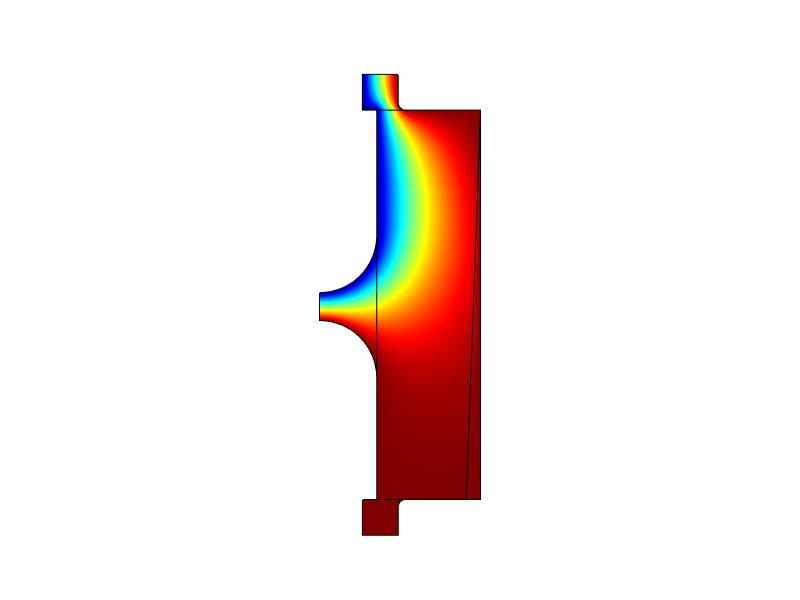
\includegraphics{figures/COMSOL_Beispielbild.jpg}		
	\caption[Kurze Abbildungsbeschreibung]{Electron drift currents in Ar at 30 Td and in CO$_2$ at 65 Td, the latter was divided by 10 and shifted by 0.2 $\mu$s. Dotted lines are averages of measured waveforms, solid lines are fits of Eq. XX. $T$ marks the electron transit time, and the markers $T_1$ to $T_3$ are explained in section.} %\ref{sec.analysecurrent}
	\label{fig.waveforms}
\end{figure}
Averaged electron current waveforms $I_e$ are aquired, of which two examples are shown in figure \ref{fig.waveforms}.
The initial broadening of the swarm $\sigma_0$ and its starting time $t_0$ are obtained by fitting a Gaussian to the rising edge of $I_e$. A tentative fit of equation XX with four free parameters to the whole waveform produces preliminary values $n_0, T, \nu_{\mathrm{eff}}, \tau_{\mathrm{D}}$. Using these preliminary values the waveform is partitioned into intervals, which are individually analysed by fitting expressions of only two free parameters. From the interval $T_1$ to $T_2$, as shown in figure \ref{fig.waveforms}
, the definitive values $n_0$ and $\nu_{\mathrm{eff}}$ are obtained, and from the interval $T_2$ to $T_3$ follows $T$ and $\tau{_\mathrm{D}}$.

This analysis relates one set of temporal parameters $(T, \nu_{eff}, \tau_{D})$ to one set of experiment parameters $(N, d, U)$.

We used Physics to solve problems